\documentclass[11pt]{article}

\newcommand{\csim}{\textsf{CSIM} }
\newcommand{\nmc}{\textsf{Circuit-Tool} }
\newcommand{\lsm}{\textsf{Learning-Tool} }

%
% common packages 
%
\usepackage{graphicx}
\usepackage{color}

\PassOptionsToPackage{colorlinks=true,linkcolor=blue,citecolor=blue,urlcolor=blue}{hyperref}

\usepackage{html}

%begin{latexonly}
\usepackage{a4wide}
%\newif\ifpdf\ifx\pdfoutput\undefined\pdffalse\else\pdfoutput=1\pdftrue\fi
%\newcommand{\pdfgraphics}{\ifpdf\DeclareGraphicsExtensions{.pdf,.jpg}\else\DeclareGraphicsExtensions{.eps}\fi}
%\newcommand{\pdfgraphics}{}
%\ifpdf
%\else
% \usepackage[dvips]{hyperref}
%\fi
%end{latexonly}

\html{
  \pagecolor[gray]{1.0}
%  \newcommand{\pdfgraphics}{}
  \newcommand{\href}[2]{\htmladdnormallink{#2}{#1}}
  % we assume that the name of the hypertarget also exists as label!
  \newcommand{\hyperlink}[2]{\hyperref{#2}{}{}{#1}} 
  \newcommand{\hypertarget}[2]{#2}
}

\newcommand{\Section}[2]{\hypertarget{#2}{\section{#1}\label{#2}}}
\newcommand{\Subsection}[2]{\hypertarget{#2}{\subsection{#1}\label{#2}}}
\newcommand{\Subsubsection}[2]{\hypertarget{#2}{\subsubsection{#1}\label{#2}}}

\newcommand{\secref}[2]{\hyperlink{#1}{#2}\latex{ (Sec.~\ref{#1})}}
\newcommand{\sect}[1]{\hyperlink{#1}{Section}~\ref{#1}}
\newcommand{\figref}[1]{\hyperlink{#1}{Figure}~\ref{#1}}

\setlength{\parindent}{0em}
\setlength{\parskip}{1ex plus 0.1ex minus 0.1ex}
\setlength{\itemsep}{-0.5ex plus 0.1ex minus 0.1ex}
\setlength{\topmargin}{0cm}

%
% since we include the detailed description from doxygen we need some
% of these definitions
%
\input{doxygen}

%
% define the \objfield which is output by reggen for each registered
% field of an object.
%
\newcommand{\objfield}[6]{\item[{\normalsize \texttt{#2}} ($ #5 $) :]  {\small #6}}
\newcommand{\objfieldnu}[6]{\item[{\normalsize \texttt{#2}} :] {\small #6}}
\newcommand{\cmdref}[1]{\Subsubsection{#1}{cmd:#1}}
  
\begin{document}
%\pdfgraphics
\sloppy

%
% titlepage 
%
\latex{{
\begin{center}
  \thispagestyle{empty}
  \Huge
  
  \rule{0cm}{0cm}\\ \vfill
  
  \textbf{\csim: A Neural \textit{C}ircuit \textit{SIM}ulator}\\
  {\Large Version 1.1} \\
  \textbf{User Manual}
  
  \Large
  \vspace{3cm}
  \copyright 2002 The IGI LSM Group\\
  \url{www.lsm.tugraz.at}\\
  
  \vspace{1cm}
  
  \large
  \today
  
  \vspace{5cm}

  \vfill
  
\end{center}

% GPL
\setlength{\parindent}{0em}
\setlength{\parskip}{1ex plus 0.1ex minus 0.1ex}
\renewcommand{\baselinestretch}{0.95}
\scriptsize

This document is part of \csim Release 1.1

Copyright �2002 The IGI LSM group

\csim is free software; you can redistribute it and/or modify it
under the terms of the \href{http://www.gnu.org/copyleft/gpl.html}{GNU
  General Public License} as published by the Free Software
Foundation; either version 2, or (at your option) any later version.

\csim is distributed in the hope that it will be useful, but WITHOUT
ANY WARRANTY; without even the implied warranty of MERCHANTABILITY or
FITNESS FOR A PARTICULAR PURPOSE. See the GNU General Public License
for more details.

To get a copy of the GNU General Public License point your browser to
\url{http://www.gnu.org/copyleft/gpl.html}.

The IGI LSM group\\
Institute for Theoretical Computer Science\\
Graz University of Technology\\
Inffeldgasse 16/b, A-8010 Graz, AUSTRIA\\
\url{lsm@igi.tu-graz.ac.at}, \url{www.lsm.tugraz.at}

}
\clearpage
}
\html{\begin{flushleft}
{  \Huge  
  \textbf{\csim: User Manual}\\
  {\Large CSIM Version 1.1} \\
}

This manual is intended to describe how to use \csim from the (Matlab)
users point of view. It \emph{does not} try to explain (or give an
introduction to) the type of models which can be simulated with CSIM.
Regarding neural modeling we refer the reader to \cite{DayanAbbott:01}
and \cite{GerstnerKistler:02}.  Furthermore
\href{http://www.mathworks.com}{Matlab} programming knowledge is
assumed.

\html{This manual is also available as \href{usermanual.pdf}{printable
PDF file}.}

\latex{This manual is also available in \href{usermanual.html}{HTML
format}.}


\end{flushleft}

}

%
% table of contents
%
%%%%%%%%%%%%%%%%%%%%%%%%%%%%%%%%%%%%%%%%%%%%%%%%%%%%%%%%%%%%%%%%%%%%%%%

\setcounter{tocdepth}{3}
\tableofcontents

%%%%%%%%%%%%%%%%%%%%%%%%%%%%%%%%%%%%%%%%%%%%%%%%%%%%%%%%%%%%%%%%%%%%%%%

\Section{Preliminaries}{sec:pre}

\input{prelim}

%%%%%%%%%%%%%%%%%%%%%%%%%%%%%%%%%%%%%%%%%%%%%%%%%%%%%%%%%%%%%%%%%%%%%%%

\clearpage

\Section{A short Tutorial}{sec:start}


In this section we will introduce \csim by means of a simple example.
We will use \csim to simulate a model where a
\secref{classLifNeuron}{leaky-integrate-and-fire} neuron (LIF neuron)
is driven by a Poisson spike train which is transmitted by a
\secref{classDynamicSpikingSynapse}{dynamic synapse}.

\begin{center}
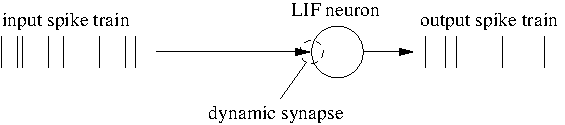
\includegraphics{first-model}
\end{center}

%\Subsection{Setting up the simulation}{subsec:setup}

\subsection{Creating Objects}

Each element/entity of the simple model we will implement, will be
simulated by a corresponding \emph{object} in \csim. The following
table shows the correspondence between the elements of the model and
the \emph{class} of the object used to simulate the element
%
\begin{center}
\begin{tabular}{l|l}
\textbf{element of model} & \textbf{class of \csim object} \\\hline
input spike train & \texttt{SpikingInputNeuron} \\
dynamic synapse & \texttt{DynamicSpikingSynapse} \\
LIF neuron & \texttt{LifNeuron}
\end{tabular}
\end{center}
%
Hence, for the simulation to run one must \secref{cmd:create}{create
  objects} of the given class:
%
\begin{tabbing}
\quad\tt>> i=csim('create','SpikingInputNeuron'); \\
\quad\tt>> s=csim('create','DynamicSpikingSynapse'); \\
\quad\tt>> n=csim('create','LifNeuron');
\end{tabbing}
%

\subsection{Object Handles}

The values \texttt{i, s}, and \texttt{n} returned by these
\secref{cmd:create}{create commands} are the \emph{indices} or
\emph{handles} to the created objects. The handles are the only means
to further access or modify existing objects.

\subsection{Setting Fields or Parameters}

Each of the created objects has several \emph{fields} which usually
correspond to a parameter of the model which is implemented by the
class of the object. To display for example all
\secref{classLifNeuron}{fields of the \texttt{LifNeuron}} object we
can use the command
%
\begin{tabbing}
\quad\tt>> csim('\hyperlink{cmd:get}{get}',n);
\end{tabbing}
%
This will yield the following output
%
\begin{verbatim}
  0 : LifNeuron
          Cm = 3e-08 (F)
          Rm = 1e+06 (Ohm)
    Vresting = -0.06 (V)
      Vreset = -0.06 (V)
       Vinit = -0.06 (V)
    Trefract = 0.003 (sec)
      Inoise = 0 (A)
     Iinject = 0 (A)
     Vthresh = -0.045 (V)
          Vm : 0 (V)
        type = 0
     nSpikes : 0
   nIncoming : 0
   nOutgoing : 0
\end{verbatim}
%
Some of the fields are parameters of the model (\texttt{Cm},
\texttt{Rm}, ...) which can be modified (denoted by the \texttt{'='})
others are internal state variables (\texttt{Vm} in this case) which
can not be changed (denoted by the \texttt{':'}) and yet other provide
auxiliary information (\texttt{nSpikes}, \texttt{nIncoming}, ...). See
the \secref{sec:clref}{Class Reference} for details about fields
of a particular object.

Suppose we want to change the absolut refractory period of the LIF
neuron \texttt{n} to be of length 2\,ms and add a noisy current of
50\,nA. This can be done with the command
%
\begin{tabbing}
\quad\tt>> csim('\hyperlink{cmd:set}{set}',n,'Trefract',0.002,'Inoise',50e-9);
\end{tabbing}
%
For the dynamic synapse \texttt{s} we choose parameters such that it
will show a depressing behaviour:
%
\begin{tabbing}
\quad\tt>> csim('\hyperlink{cmd:set}{set}',s,'W',10,'U',0.1,'D',1,'F',0.05); \\
\quad\tt>> csim('\hyperlink{cmd:set}{set}',s,'u0',0.1,'r0',1);
\end{tabbing}

\subsection{Making connections}
So far we have generated three independent objects and set
their fields to the desired values. Now we have to connect the objects
to implement our simple model. We have to connect the input \texttt{i}
to the synapse \texttt{s} and the synapse to the neuron \texttt{n}:
%
\begin{tabbing}
\quad\tt>> csim('\hyperlink{cmd:connect}{connect}',n,s); \% synapse to neuron \\
\quad\tt>> csim('\hyperlink{cmd:connect}{connect}',s,i); \% input to synapse
\end{tabbing}
%
Note the the \secref{cmd:connect}{connect command} uses the convention
that the signal destination is the first argument. Alternatively one
can use the three argument form of the command:
\begin{tabbing}
\quad\tt>> csim('\hyperlink{cmd:connect}{connect}',n,i,s); \% input to neuron via synapse
\end{tabbing}

\subsection{Recording}  The model is now fully
implemented. In addition we want to record traces of some quantities
of interest. Suppose we want record the membrane potential and the
spikes of neuron \texttt{n} as well as the postsynaptic respones (the
field \texttt{psr}) of the synapse. To do so we have to create a
\secref{classRecorder}{Recorder object} and tell this object which
fields from which objects to record. The recorder is created with the
command
%
\begin{tabbing}
\quad\tt>> r=csim('\hyperlink{cmd:create}{create}','Recorder');
\end{tabbing}
%
and the following commands tell the recorder \texttt{r} to record the
field \texttt{psr} of synapse \texttt{s} as its first trace and the
field \texttt{Vm} of neuron \texttt{n} as its second trace:
%
\begin{tabbing}
\quad\tt>> csim('\hyperlink{cmd:connect}{connect}',r,s,'psr'); \\
\quad\tt>> csim('\hyperlink{cmd:connect}{connect}',r,n,'Vm');   \\
\end{tabbing}
%
Using the special field \texttt{spikes} the same syntax will be used
to record the spikes of neuron \texttt{n} as the third trace of
recorder \texttt{r}.
\begin{tabbing}
\quad\tt>> csim('\hyperlink{cmd:connect}{connect}',r,n,'spikes');
\end{tabbing}

The following figure summarizes which objects we have created and how
they are connected:

\begin{center}
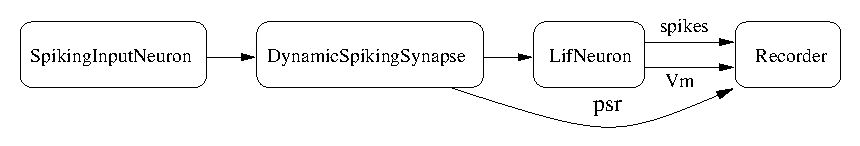
\includegraphics{first-model-csim}
\end{center}

\subsection{Setting up the input} Before we are ready to run the
simulation we have to define the spike train which should be emitted
 by the input neuron \texttt{i}. In \csim time varying
 \secref{sec:inputs}{\emph{input signals}} (analog or spiking) -- also
 called the \emph{stimulus} -- are not considered to be
 properties/attributes of some objects but are always explicitly
 specified. In the case of our example we will define a spike train
 with randomly drawn spike times (for details see \sect{sec:inputs}):
\begin{tabbing}
\quad\tt>> S.spiking = 1;                \% 1 ... spike times, 0 ... analog data\\
\quad\tt>> S.dt      = NaN;              \% resolution for analog data \\
\quad\tt>> S.idx     = i;                \% index/handle of receiving object\\
\quad\tt>> S.data    = sort(rand(1,10)); \% 10 random spikes in the interval 0 to 1 sec
\end{tabbing}

\subsection{Running the simulation} Now we are ready to run the
simulation. The command
%
\begin{tabbing}
\quad\tt>> Tsim=1; \\
\quad\tt>> csim('\hyperlink{cmd:simulate}{simulate}',Tsim,S);
\end{tabbing}
%
simulates the simple model for 1\,sec starting at time
$t=0$\footnote{In general the simulation will be continued at the time
where the last \secref{cmd:simulate}{simulate command}
stopped. However the first simulate command -- as in the case of the
example -- starts at time $t=0$. Simulation time can be reset to time
$t=0$ with the \secref{cmd:reset}{reset command}
\texttt{csim('reset');}.} with the stimulus \texttt{S}.

\subsection{Plotting the recorded traces} The traces recorded by the
recorder can be obtained by the command
\begin{tabbing}
\quad\tt>> t=csim('\hyperlink{cmd:get}{get}',r,'traces')
\end{tabbing}
which yields the output
\begin{verbatim}
t = 
    channel: [1x3 struct]
\end{verbatim}
A closer look at e.g. the first channel reveals that
\texttt{t.channel} is a struct array with a similar structure as we
have seen above for the input signal:
\begin{verbatim}
>> t.channel(1)           

ans = 

          idx: 1
    fieldName: 'psr'
         data: [1x2000 double]
      spiking: 0
           dt: 5.0000e-04
\end{verbatim}

The output indicates that \texttt{t.channel(1).data} holds the
\texttt{psr} trace (\texttt{t.channel(1).fieldName}) with a resolution
of 0.5\,ms (\texttt{t.channel(1).dt}). See the
\secref{classRecorder}{Recorder class documentation} for details abput
the structure of the trace output. Similarly \texttt{t.channel(2)}
holds the the \texttt{Vm} trace and \texttt{t.channel(3)} holds the
output spike times. Hence the following command will plot
the \texttt{psr} trace
\begin{tabbing}
\quad\tt>> plot(t.channel(1).dt:t.channel(1).dt:Tsim,t.channel(1).data);
\end{tabbing}
and the command
\begin{tabbing}
\quad\tt>> stem(t.channel(3).data,ones(size(t.channel(3).data)));
\end{tabbing}
will draw the output spike train.

Using another set of plot commands one can easily create the following
figure which shows the input, the postsynaptic response and the output
of the neuron (the voltage and the spikes)

\begin{center}
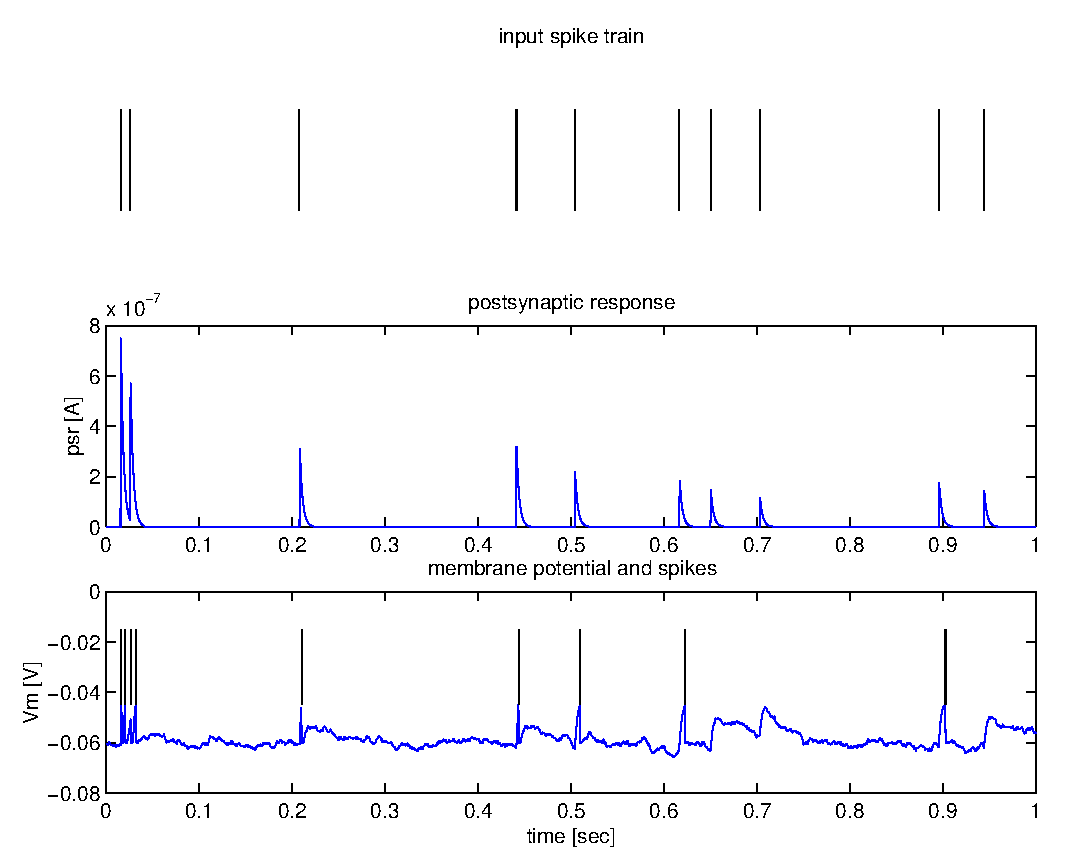
\includegraphics[width=12cm]{first-model-output}
\end{center}

The full code of this example is contained as the file
\texttt{first\_model.m} in the demo directory of the
\href{http://www.lsm.tugraz.at/csim}{\csim package}.




%%%%%%%%%%%%%%%%%%%%%%%%%%%%%%%%%%%%%%%%%%%%%%%%%%%%%%%%%%%%%%%%%%%%%%%

\Section{Input and Output}{sec:inout}

\Subsection{Input Signals}{sec:inputs}

% \Subsubsection{Single-stimulus input}{sec:singlein}

When runing a network simulation via \texttt{csim('simulate',...);}
one can specify \emph{input signals} like in the command
%
\begin{tabbing}
\quad\texttt{>> csim(\hyperlink{cmd:simulate}{'simulate'},Tsim,S);}
\end{tabbing}
%
where \texttt{S} is a struct array with the following fields:
%
\begin{itemize}
  
\item \texttt{S(i).idx} : array of handles of objects which should
  receives this signal

\item \texttt{S(i).spiking} : binary flag (0/1) which determines if
  \texttt{S(i).data} should be interpreted as spike times or as an
  analog signal
  
\item \texttt{S(i).dt} : time discretization; for analog signals
  (\texttt{S(i).spiking}=0) only
  
\item \texttt{S(i).data} : signal data: vector of the analog values
  (\texttt{S(i).spiking}=0) or spike times (\texttt{S(i).spiking}=1)

\end{itemize}
%
Note that \texttt{csim('simulate',...);} accepts an arbirary number of
such struct arrays. See \secref{cmd:simulate}{documentation of the
  simulate command}.


%\Subsubsection{Multi-stimulus input}{sec:multiin}
%
%When runing a network simulation via \texttt{csim('simulate',...);}
%one can specify a \emph{multi-stimulus} input \texttt{S} like in the command
%
%\begin{tabbing}
%\quad\texttt{>> R = csim(\hyperlink{cmd:simulate}{'simulate'},Tsim,S);}
%\end{tabbing}
%
%where \texttt{S} is a $n \times 1$ struct array of the form
%\texttt{S(i).channel} which describes the $i$-th stimulus.
%\texttt{S(i).channel} has the structure as described above.
%
%If such multi-stimulus input is specified \csim will simulate the
%current network with each of the $n$ stimuli where at the beginning of
%each stimuli the network is reset to $t=0$. The return argument
%\texttt{R} contains the recorded information of all $n$ simulations
%(see \sect{sec:multiout}).


\Subsection{Output}{sec:output}

If one simulates a network then one also wants to record the
quantities of interest. In our \secref{sec:start}{introductory
  example} we were interested in the membrane potential of the
leaky-integrate and fire neuron. \csim can record any field of any
object by means of \secref{classRecorder}{Recorder} objects. The
following code fragment shows how to set up a Recorder to record the
membrane potential (\texttt{Vm}) of a
\secref{classLifNeuron}{LifNeuron} object with handle \texttt{n}.
%
\begin{tabbing}
\quad\texttt{>> rec = csim(\hyperlink{cmd:create}{'create'},'\hyperlink{classRecorder}{Recorder}');} \\
\quad\texttt{>> csim(\hyperlink{cmd:connect}{'connect'},rec,n,'Vm');}
\end{tabbing}
%
Note that one Recorder object can record an arbitrary number of
fields from arbitrary objects.

\Subsubsection{Getting results of the last simulation}{sec:lastout}

After a network simulation via a command like
%
\begin{tabbing}
\quad\texttt{>> csim(\hyperlink{cmd:simulate}{'simulate'},Tsim,\hyperlink{sec:input}{InputSignal});}
\end{tabbing}
%
the recorded data of the \emph{the last simulation} Recorder
\texttt{rec} can be obtained by the command
\begin{tabbing}
\quad\texttt{>> R=csim(\hyperlink{cmd:get}{'get'},rec,'traces');}
\end{tabbing}
The exact structure of \texttt{R} for the recorder \texttt{rec}
depends on the value of the \secref{classRecorder}{field
\texttt{commonChannels} of the \texttt{Recorder}} object.


\paragraph{\texttt{commonChannels = 0}} In this case  (default) \texttt{R}
is a struct array with the only field \texttt{channel} which is in
turn a struct array with a similar structure as an
\secref{sec:inputs}{input signal}. That is

\begin{itemize}
  
\item \texttt{R.channel(j).idx} : handle of the object from which
  field the data was recorded
  
\item \texttt{R.channel(j).spiking} : binary flag (0/1) which
  determines if \texttt{data} should be interpreted as spike times or
  as an analog signal
  
\item \texttt{R.channel(j).dt} : time discretization; for analog
  signals   only
  
\item \texttt{R.channel(j).data} : signal data : vector of the
  analog values or spike times. Note that the data always starts at
  time $t=0$.
 
\item \texttt{R.channel(j).fieldName} : name of the recorded
    field

\end{itemize}

\paragraph{\texttt{commonChannels = 1}} In this case
\texttt{R} has two fields:
\begin{itemize}
\item \texttt{R.data} : A double array where
  \texttt{R.data(j,s)} is the $s$-th recorded value of the $j$-th
  field recorded.  Note that the data always
  starts at time $t=0$.  {\small Remark: The number of values which
    are recorded depends on the \secref{classRecorder}{field
      \texttt{dt} of the \texttt{Recorder} object}.}
  
\item \texttt{R.info} : A struct array where
  \texttt{R.info(j).idx} is the handle of the object from which
  the field \texttt{R.info(j).fieldName} is recorded.
\end{itemize}

\Subsubsection{Getting the results of a multi-stimulus simulation}{sec:multiout}

{\bf Reminder}: The command
\begin{tabbing}
\quad\texttt{>> R=csim(\hyperlink{cmd:get}{'get'},rec,'traces');}
\end{tabbing}
returns only the results of the last simulation. In the case of a
multi-stimulus simulation with stimulus array \texttt{S} of length $n$
this command returns only the result of the simulation with stimulus
\texttt{S(n)}.

To get the results of all $n$ simulations one has to use
\begin{tabbing}
\quad\texttt{>> R=csim(\hyperlink{cmd:simulate}{'simulate'},Tsim,S);}
\end{tabbing}

In that case \texttt{R} contains the results of all $n$ stimulations.
\texttt{R\{r\}(s).channel} contains the recorded data of the $r$-th
recorder during the $s$-th simulation ($1 \leq s \leq n$).
\texttt{R\{r\}(s).channel} is of the format as described in
\sect{sec:lastout}.





 
%%%%%%%%%%%%%%%%%%%%%%%%%%%%%%%%%%%%%%%%%%%%%%%%%%%%%%%%%%%%%%%%%%%%%%%
%
%\Section{Distributed Simulation}{sec:distr}
%
%\input{distributed}
% 

%%%%%%%%%%%%%%%%%%%%%%%%%%%%%%%%%%%%%%%%%%%%%%%%%%%%%%%%%%%%%%%%%%%%%%%

\Section{Additional Topics}{sec:additional}

\subsection{How the network is simulated}

\csim employs a fixed time step simulation scheme for the
integration of the differential equations involved (represented by
objects). Currently all objects use the exponential Euler method with
the same integration time step (see \sect{sec:gf}).

During each time step a certain method (\texttt{advance}) is called
for each object part of the simulation. There is a fixed schedule
which depends a) on the class of the object and b) on the time of
creation. Here is the order of the classes.
%
\begin{enumerate}
\item Neuron
\item Synapse
\item Recorder
\end{enumerate}
%
This means that all objects of classes derived from a generic Neuron
are advanced first followed by objects of classes derived from a generic
Synapse and so on.

Note that for example a more detailed neuron model (like the
\secref{classCbNeuron}{CbNeuron}) has to advance all its child objects
like ion channels.

After a \texttt{csim('simulate',...)} command returns the network is
kept in its current state at this time $t$. A further
\texttt{csim('simulate',...)}  command continues the simulation at
this time $t$. Use \texttt{csim('reset');} to reset the simulation to
time $t=0$.

Note that recorded traces you get by the appropriate
\secref{cmd:get}{get command} always start at time $t=0$.


\Subsection{Global fields}{sec:gf}

There are a few fields which determine the global (i.e. not object
specific) behavior of \csim which can be modified via the
\secref{cmd:set}{set command}:
%
\begin{tabbing}
\quad\tt>> csim('\hyperlink{cmd:set}{set}',<fieldname>,<value>); \\
\end{tabbing}
%

\subsubsection*{Read/writeable fields}


\begin{description}

\item[dt] The integration time step used by all objects

\item[randSeed] The seed value for the random number generator

\item[verboseLevel] How much stuff should be written to the
  console window (no effect yet!).
  
\item[nThreads] Number of threads to use for simulation (no
  effect yet!). The multi-threaded version of \csim is currently under
  development.

\item[spikeOutput] Flag: 1 ... always output spikes as last cell element, 0 do not
  output spikes (obsolete).

\end{description}

\subsubsection*{The following fields are read-only:}

\begin{description}

\item[t] The current virtual (simulation) time
  
\item[step] The current time step; i.e.  \texttt{step=t/dt};

\end{description}

\subsection{Event driven simulation}

Since in a typical simulation the firing rate of the neurons is about
30\,Hz and the time constant of a synaptic current is typically about
3\,ms most of the time a synapse is ``idle''. This observation
encouraged us to implement some ideas of event driven simulators like
\href{http://www.cnl.salk.edu/~arno/spikenet/}{SpikeNet}\latex{\footnote{\url{http://www.cnl.salk.edu/~arno/spikenet/}}}:
We decided to cut off the very far tail of the exponential decaying
synaptic responses (after 5 time constants) and remove those synapses
from the list of active synapses (which are advanced every time step).
A synapse is re-activated if it receives a further spike. For large
networks with lots of synapses these idea results in an average
speed-up of 2 to 3.


 
%%%%%%%%%%%%%%%%%%%%%%%%%%%%%%%%%%%%%%%%%%%%%%%%%%%%%%%%%%%%%%%%%%%%%%%

\Section{Adding your own C++ model classes to \csim}{sec:usermodels}

\input{usermodels}
 
%%%%%%%%%%%%%%%%%%%%%%%%%%%%%%%%%%%%%%%%%%%%%%%%%%%%%%%%%%%%%%%%%%%%%%%

\clearpage

\Section{\csim command reference}{sec:cmdref}


The common form of all \csim commands is 
\begin{verbatim}
  csim(command,...);
\end{verbatim}
where \texttt{command} is one of the following strings:

\begin{itemize}
\setlength{\itemsep}{-0.8ex plus 0.1ex minus 0.1ex}
\setlength{\parsep}{0.0ex plus 0.1ex minus 0.1ex}
\item \texttt{\secref{cmd:create}{'create'}} : Create an object of a certain class
\item \texttt{\secref{cmd:set}{'set'}} : Set fields of an object
\item \texttt{\secref{cmd:connect}{'connect'}} : Connect objects
\item \texttt{\secref{cmd:get}{'get'}} : Get field values of an object
% \item \texttt{\secref{cmd:access}{'access'}} : Set default network
\item \texttt{\secref{cmd:reset}{'reset'}} : Reset the simulation to $t=0.0$
\item \texttt{\secref{cmd:simulate}{'simulate'}} : Simulate the network
\item \texttt{\secref{cmd:export}{'export'}} : Export the network for saving it
\item \texttt{\secref{cmd:import}{'import'}} : Import a loaded network
\item \texttt{\secref{cmd:destroy}{'destroy'}} : Destroy/delete the current netork
\item \texttt{\secref{cmd:list}{'list'}} or \texttt{\secref{cmd:list}{'ls'}} List various items
\item \texttt{\secref{cmd:version}{'version'}} : Print out a version string
% \item \texttt{\secref{cmd:pvm}{'pvm'}} : Initialize distributed simulation
\end{itemize}

A detailed description of each of the commands follows. 

%\subsection{Multiple Networks}
%
%\csim is capable of holding more then one network at a time. There are
%two ways of specifing on which network a command should operate.
%
%\begin{itemize}
%\item For each command of the form \texttt{csim(command,...);} the
%form \texttt{csim(netIdx,command,...);} exists which allows you to
%explicitly specify the network to operate on.
%
%\item If \texttt{csim(command,...);} is used the \emph{default
%    network} is used. The default network is set using the command
%  \texttt{csim('access',netIdx);}.
%\end{itemize}
%
%\cmdref{access}
%
%\begin{itemize}
%  
%\item \texttt{idx=csim('access',netIdx);} makes the network specified
%  by \texttt{netIdx} the default network and returns that value.%
%
%\item \texttt{csim('access',netIdx);} makes the network specified
%  by \texttt{netIdx} the default network and prints that value.
%
%\item \texttt{idx=csim('access');} returns the index of the default
%  network.
%
%\item \texttt{csim('access');} prints the index of the default%
%
%\end{itemize}


\subsection{Setting up a network simulation}

\cmdref{create}

\begin{itemize}
  
%\item \texttt{idx=csim('create','Network');} creates a new network and
%  returns the \emph{index} or \emph{handle} for the created network.
%  The new network is the new default network; see command
%  \secref{cmd:access}{access}.

\item \texttt{idx=csim('create',class);} creates an object of the class
  specified by the string \texttt{class} and returns a \texttt{uint32}
  \emph{index} or \emph{handle} for the created object. This
  index/handle is the only means to access the created object.
  
\item \texttt{idx=csim('create',class,N);} creates \texttt{N} objects
  of the class specified by the string \texttt{class} and returns a
  \texttt{uint32} vector of indices/handles for the created objects.

\end{itemize}

The handles returned by \texttt{idx=csim('create',...);} are used to
identify the objects later in \texttt{'set'}, \texttt{'get'} and
\texttt{'connect'} calls.

See the \secref{sec:clref}{Class Reference} for a full description of
all available classes.

\cmdref{set}

\begin{itemize}
  
\item \texttt{csim('set',field,value);} sets the
  \secref{sec:gf}{network field} specified by the string
  \texttt{field} to \texttt{value}.
  
\item \texttt{csim('set',idx,field,value);} sets the field specified
  by the string \texttt{field} of the object with index/handle
  \texttt{idx} to \texttt{value}. \texttt{idx} can also be a vector
  of indices/handles of objects of the same class.
  
If \texttt{idx} is a vector and \texttt{value} is a scalar then the
fields of all objects are set to \texttt{value}.

If \texttt{idx} and \texttt{value} are vectors of the same size then
the field \texttt{field} of all objects \texttt{idx(i)} is set to
\texttt{value(i)}.

\item \texttt{csim('set',idx,f1,v1,f2,f2,...,fn,vn);} sets the fields
  specified by the strings \texttt{f1}, \texttt{f2}, ..., \texttt{fn}
  of the object with index/handle \texttt{idx} to the values
  \texttt{v1}, \texttt{v2}, ... \texttt{vn}. \texttt{idx} and
  \texttt{v1}, \texttt{v2}, ... \texttt{vn} can also be vectors.

\end{itemize}


\cmdref{connect}

\begin{itemize}
  
\item\texttt{csim('connect',dstIdx,srcIdx);} sets up a signal flow
  from the source \texttt{srcIdx} object (e.g. a synapse) to the
  destination object \texttt{dstIdx} (e.g. the postsynaptic neuron)
  where \texttt{dstIdx} and \texttt{srcIdx} are indices/handles to
  objects.
  
  \texttt{dstIdx} and \texttt{srcIdx} can also be vectors. In that
  case for each \texttt{i=1:length(srcIdx);} a signal flow
  $\mathtt{dstIdx(i)} \leftarrow \mathtt{srcIdx(i)}$ is set up.
  
\item\texttt{csim('connect', dstIdx, srIdx, viaIdx);} for each
  \texttt{i=1:length(srcIdx);} a signal flow of the form
  $\mathtt{dstIdx(i)} \leftarrow \mathtt{viaIdx(i)} \leftarrow
  \mathtt{srcIdx(i)}$ is set up where \texttt{dstIdx},
  \texttt{srcIdx}, and \texttt{viaIdx} are vectors of the same length
  of indices/handles to objects.
  
\item\texttt{csim('connect',recIdx,objIdx,fieldName);} connects the
  object with handle \texttt{objIdx} to the recorder with handle
  \texttt{recIdx}. The recorder \texttt{recIdx} will then record a
  trace of the values of the field \texttt{fieldName} of the objects
  specified by the vector of hadles \texttt{objIdx}.

\end{itemize}

\subsection{Running the network simulation}

\cmdref{reset}

\texttt{csim('reset');} resets the simulation time $t$ back to
$t=0.0$.

\Subsubsection{simulate}{cmd:singlesim}
\label{cmd:simulate}

\begin{itemize}
  
\item \texttt{csim('simulate',Tsim,InputSignals);} runs the network
  simulation for \texttt{Tsim} seconds starting at the time where the
  last simulate command stopped with \secref{sec:inputs}{input signals
    \texttt{InputSignals}}.
  
\item \texttt{csim('simulate',Tsim,I1,I2,...,In);} same as above but
  with input signals \texttt{I1} to \texttt{In}. There is no special
  meaning in the ordering of the input signals. It is equvivalent to
  concatenate \texttt{I1} to \texttt{In} into one struct array and
  pass this array as the single input signal.
  
\item \texttt{R=csim('simulate',Tsim,InputSignals);}\\ same as
  \texttt{csim('simulate',Tsim,InputSignals);} but in addition returns
  the cell array \texttt{R} which holds the \secref{sec:output}{output
    (traces) of all Recorder objects}.
  
\item \texttt{R=csim('simulate',Tsim,I1,I2,...,In);}\\ same as
  \texttt{csim('simulate',Tsim,I1,I2,...,In);} but in addition returns
  the cell array \texttt{R} which holds the \secref{sec:output}{output
    (traces) of all Recorder objects}.

\item \texttt{R=csim('simulate',Tsim,I1,I2,...,In);}\\ same as
  \texttt{csim('simulate',Tsim,I1,I2,...,In);} but in addition returns
  the cell array \texttt{R} which holds the \secref{sec:output}{output
    (traces) of all Recorder objects}.


\end{itemize}

%\Subsubsection{Multi-stimulus simulate}{cmd:singlemulti}
%
%\texttt{R=csim('simulate',Tsim,S);} runs $n$ network simulations for
%\texttt{Tsim} sec. The network is reset to $t=0$ before each
%simulation.
%
%The $n$ simulations are determined by the $n \times 1$ strucht array
%\texttt{S} where \texttt{S(i).channel} specifies the stimulus for the
%$i$-th simulation (see \sect{sec:multiin}).
%
%\texttt{R} contains the reorded values of all $n$ simulations (see
%\sect{sec:multiout}).
%  
%If the \secref{sec:distr}{distributed simulation} is on (see command
%\secref{cmd:pvm}{pvm}), the $n$ simulations will be carried out in
%parallel.
%
%\subsection{Initializing PVM}
%
%\cmdref{pvm}

\subsection{Saving, loading and deleting networks }

\cmdref{export}

The command
\begin{verbatim}
  net = csim('export');
\end{verbatim}
produces a struct array \texttt{net} which contains all information
about the current network simulation which is needed to set up the
simulation. Using \texttt{save file.mat net} you can save the whole
network simulation.

NOTE: The struct array \texttt{net} returned by
\texttt{net=csim('export');} is only intended to be saved to disk for
later use by \texttt{csim('import',net);} and does not have a human
readable form.

\cmdref{import}

The command
\begin{verbatim}
  csim('import',net);
\end{verbatim}
allows you to set up a network simulation from the struct array
\texttt{net} which has previously been generated by \texttt{net =
  csim('export');}. In combination with the matlab command
\texttt{load} this \csim command serves the purpose of loading a
simulation from disk.

If the current network (either explicitly specified or default
network) does not contain any objects the \texttt{net} will be
imported into that network. If there are already objects a new network
will be created and and \texttt{net} will be imported to that.

NOTE: The struct array \texttt{net} returned by
\texttt{net=csim('export');} \emph{does not} contain information about
the current state of the simulation at time $t$.  \emph{Hence it is
  only possible to start simulation based on such an arry at time
  $t=0.0$.}

\cmdref{destroy}

\texttt{csim('destroy');} all the networks.

\subsection{Displaying/Getting information}

\cmdref{get}

\begin{itemize}

  \item \texttt{csim('get');} diplays the values of the \secref{sec:gf}{global fields}

  \item \texttt{v=csim('get',field);} return the value of the
    \secref{sec:gf}{global field} specified by the string \texttt{field}

  \item \texttt{csim('get',idx);} displays the values of all fields of the
    object specified by the array index/handle \texttt{idx}

  \item \texttt{v=csim('get',idx,field);} returns a double array
   \texttt{v} where \texttt{v(:,i)} contains the values of the field
   \texttt{field} of the object with index/handle \texttt{idx(i)}.

 \item \texttt{o=csim('get',idx,'struct');} return a struct array
   describing the object specified by the index/handle
   \texttt{idx(1)}:

   \begin{itemize}
   \item \texttt{o.className} : String containing the name of class of object
   \item \texttt{o.spiking} : Double value which is 1 if the object is a
     spike emitting object (0 otherwise)
   \item \texttt{o.fields} : Cell array of strings containing the field
     names of the object
   \item and all fields with its values.
   \end{itemize}
   
 \item \texttt{[incomming,outgoing]=csim('get',idx,'connections');}
   returns the indices/handles of the incomming (i.e. input
   delivering) and outgoing (i.e. output receiving) objects of the
   object specified by the index/handle \texttt{idx}. This is
   currently only implemented for Synapses and Neurons.
   
 \item \texttt{R=csim('get',recorder\_idx,'traces');} returns the
   traces of the fields recorded by the
   \secref{classRecorder}{Recorder} object with handle
   \texttt{recorder\_idx} during the \emph{last simulation}. See the
   \secref{classRecorder}{Recorder documentation} for details about
   the format of \texttt{R}.

\end{itemize}

\cmdref{list}

\begin{itemize}
  
\item \texttt{csim('list');} and \texttt{csim('list','classes');}
  print a list of all available classes
  
\item \texttt{csim('list','classes','-fields');} prints a list of all
  available classes with information about the fields of each class.
  Read/writeable fields are marked by a '\texttt{=}' between the field
  name and its description, wheres a '\texttt{:}' denotes a read-only
  field.

\item \texttt{csim('list','objects');}  prints a list of all created
  objects

\item \texttt{csim('list','objects','-fields');} prints a list of all
  created objects and the values of its fields. Read/writeable fields
  are marked by a '\texttt{=}' between the field name and its value,
  wheres a '\texttt{:}' denotes a read-only field.

\item \texttt{csim('list','networks');}  prints a list of all networks

\item \texttt{csim('list','networks','-fields');} prints a list of all
  networks and the values of its fields. Read/writeable fields
  are marked by a '\texttt{=}' between the field name and its value,
  wheres a '\texttt{:}' denotes a read-only field.

\end{itemize}

Not that instead of \texttt{'list'} one can use \texttt{'ls'} as a
shortcut.

\cmdref{version}

\begin{itemize}
\item \texttt{csim('version')} prints a version string
\item \texttt{v=csim('version');} returns the version string
\end{itemize}

%%% Local Variables: 
%%% mode: latex
%%% TeX-master: t
%%% End: 


%%%%%%%%%%%%%%%%%%%%%%%%%%%%%%%%%%%%%%%%%%%%%%%%%%%%%%%%%%%%%%%%%%%%%%%


\Section{\csim model classe reference}{sec:clref}

\input{um_class_ref}

%%%%%%%%%%%%%%%%%%%%%%%%%%%%%%%%%%%%%%%%%%%%%%%%%%%%%%%%%%%%%%%%%%%%%%%

\bibliographystyle{apalike}

\bibliography{references}

\end{document}
